\documentclass[aspectratio=169]{beamer}

\usepackage{amsmath}
\usepackage{amssymb}
\usepackage{algorithm}
\usepackage{algpseudocode}
\usepackage{tikz}
\usepackage{listings}

\usetikzlibrary{arrows.meta, positioning, shapes.geometric}

\usetheme{Madrid}

\title{Bowyer--Watson Delaunay Triangulation}
\author{}
\institute{}
\date{}
\newcommand{\REM}[1]{}
\begin{document}

%------------------------------------------------
\begin{frame}
    \titlepage
\end{frame}

%------------------------------------------------
\begin{frame}{Delaunay Triangulation}

Given a set of points

\[
P = \{p_1,p_2,\ldots,p_n\},
\]

the \textbf{Delaunay triangulation} connects the points into triangles
such that:

\begin{block}{Delaunay Property}
The circumcircle of every triangle contains no other input point
in its interior.
\end{block}

\vspace{0.3cm}

Equivalently, for every triangle $T$,

\[
\text{Interior}(\operatorname{Circumcircle}(T))
\cap P = \emptyset.
\]

\begin{itemize}
    \item Maximizes the minimum angle of the triangles.
    \item Widely used in computational geometry.
    \item Useful in mesh generation, graphics, FEM, and geographic modeling.
\end{itemize}

\end{frame}

%------------------------------------------------
\begin{frame}{Bowyer--Watson Algorithm}

The \textbf{Bowyer--Watson algorithm} constructs a Delaunay
triangulation incrementally.

\begin{enumerate}
    \item Start with a large \textbf{super-triangle}.
    \item Insert input points one at a time.
    \item Find triangles whose circumcircles contain the new point.
    \item Remove these ``bad'' triangles.
    \item The removed triangles form a polygonal cavity.
    \item Connect the new point to the boundary of the cavity.
    \item Remove triangles connected to the super-triangle.
\end{enumerate}

\begin{center}
\[
\boxed{\text{Find bad triangles}
\rightarrow
\text{Remove}
\rightarrow
\text{Retriangulate}}
\]
\end{center}

\end{frame}

%------------------------------------------------
\begin{frame}{High-Level View}

\begin{center}
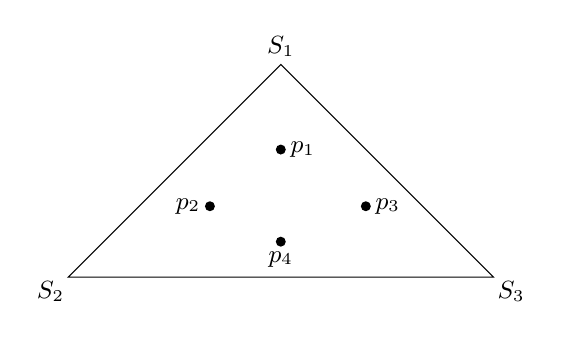
\begin{tikzpicture}[
    scale=0.9,
    every node/.style={font=\small}
]

% Super triangle
\coordinate (A) at (0,3);
\coordinate (B) at (-3,0);
\coordinate (C) at (3,0);

\draw (A)--(B)--(C)--cycle;

\node at (0,3.25) {$S_1$};
\node at (-3.25,-0.2) {$S_2$};
\node at (3.25,-0.2) {$S_3$};

% Points
\fill (0,1.8) circle (2pt) node[right] {$p_1$};
\fill (-1,1) circle (2pt) node[left] {$p_2$};
\fill (1.2,1) circle (2pt) node[right] {$p_3$};
\fill (0,0.5) circle (2pt) node[below] {$p_4$};

\end{tikzpicture}
\end{center}

\vspace{0.2cm}

The super-triangle contains all input points.

\begin{block}{Why a super-triangle?}
It provides an initial triangulation and avoids special handling
when the first points are inserted near the convex hull.
\end{block}

\end{frame}

%------------------------------------------------
\begin{frame}{Step 1: Insert a New Point}

Suppose a new point $p$ is inserted.

\begin{center}
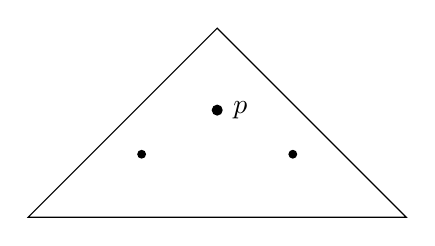
\begin{tikzpicture}[scale=0.8]

\coordinate (A) at (0,3);
\coordinate (B) at (-3,0);
\coordinate (C) at (3,0);

\draw (A)--(B)--(C)--cycle;

\fill (0,1.7) circle (2.5pt);
\node[right] at (0.1,1.7) {$p$};

\fill (-1.2,1) circle (2pt);
\fill (1.2,1) circle (2pt);

\end{tikzpicture}
\end{center}

For every existing triangle $T$, test:

\[
p \in \operatorname{Circumcircle}(T)?
\]

If yes, then $T$ is a \textbf{bad triangle}.

\end{frame}

%------------------------------------------------
\begin{frame}{Step 2: Find Bad Triangles}

For a triangle $T$ with circumcenter $c$ and radius $r$:

\[
\|p-c\|^2 < r^2
\]

means that $p$ lies inside the circumcircle.

\begin{center}
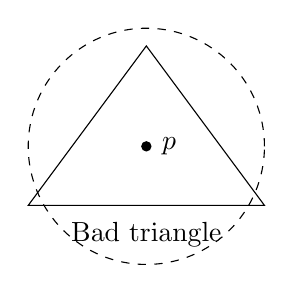
\begin{tikzpicture}[scale=0.75]

% Triangle
\coordinate (A) at (0,2.7);
\coordinate (B) at (-2,0);
\coordinate (C) at (2,0);

\draw (A)--(B)--(C)--cycle;

% Circumcircle
\draw[dashed] (0,1) circle (2);

% point
\fill (0,1) circle (2.5pt);
\node[right] at (0.1,1) {$p$};

\node at (0,-0.5) {Bad triangle};

\end{tikzpicture}
\end{center}

The triangle must be removed because it violates the Delaunay property
after inserting $p$.

\end{frame}

%------------------------------------------------
\begin{frame}{Step 3: The Cavity}

Suppose several triangles have circumcircles containing $p$.

These triangles are removed.

\begin{center}
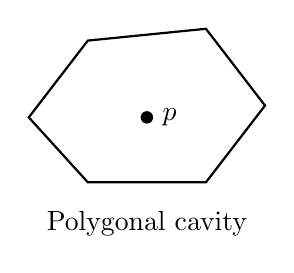
\begin{tikzpicture}[scale=0.75]

% cavity boundary
\draw[thick]
    (-2,1) --
    (-1,2.3) --
    (1,2.5) --
    (2,1.2) --
    (1,-0.1) --
    (-1,-0.1) -- cycle;

% point
\fill (0,1) circle (3pt);
\node[right] at (0.1,1) {$p$};

\node at (0,-0.8) {Polygonal cavity};

\end{tikzpicture}
\end{center}

The union of the bad triangles forms a cavity.

\vspace{0.2cm}

Only the \textbf{boundary edges} of the cavity are needed for
retriangulation.

\end{frame}

%------------------------------------------------
\begin{frame}{Step 4: Find the Cavity Boundary}

Consider two bad triangles sharing an edge.

\begin{center}
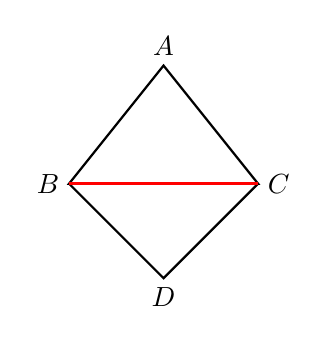
\begin{tikzpicture}[scale=0.6]

\coordinate (A) at (0,2.5);
\coordinate (B) at (-2,0);
\coordinate (C) at (2,0);
\coordinate (D) at (0,-2);

\draw[thick] (A)--(B)--(C)--cycle;
\draw[thick] (B)--(D)--(C);

\draw[red,very thick] (B)--(C);

\node[above] at (A) {$A$};
\node[left] at (B) {$B$};
\node[right] at (C) {$C$};
\node[below] at (D) {$D$};

\end{tikzpicture}
\end{center}

The edge $BC$ occurs in \textbf{two bad triangles}.

Therefore it is an \textbf{internal edge} of the cavity and is discarded.

\begin{block}{Boundary rule}
An edge appearing only once among the bad triangles belongs
to the cavity boundary.
\end{block}

\end{frame}

%------------------------------------------------
\begin{frame}{Step 5: Retriangulate the Cavity}

After removing the bad triangles, connect the new point $p$
to every boundary edge.

\begin{center}
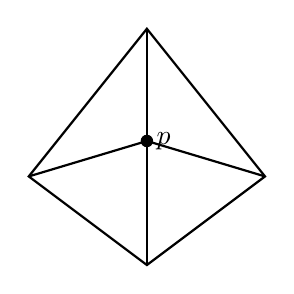
\begin{tikzpicture}[scale=0.75]

\coordinate (A) at (0,2.5);
\coordinate (B) at (-2,0);
\coordinate (C) at (2,0);
\coordinate (D) at (0,-1.5);

\coordinate (P) at (0,0.6);

\draw[thick] (A)--(B)--(D)--(C)--cycle;

\draw[thick] (P)--(A);
\draw[thick] (P)--(B);
\draw[thick] (P)--(C);
\draw[thick] (P)--(D);

\fill (P) circle (3pt);
\node[right] at (P) {$p$};

\end{tikzpicture}
\end{center}

Each boundary edge $(u,v)$ generates a new triangle:

\[
(u,v,p).
\]

\end{frame}

%------------------------------------------------
\begin{frame}{Complete Bowyer--Watson Algorithm}
\begin{algorithm}[H]
\scriptsize
\caption{Bowyer--Watson}
\begin{algorithmic}[1]

\State Create a super-triangle $ST$
\State $T \gets \{ST\}$

\ForAll{points $p$}
    \State $Bad \gets \emptyset$
    \ForAll{triangles $t \in T$}
        \If{$p$ lies inside circumcircle of $t$}
            \State $Bad \gets Bad \cup \{t\}$
        \EndIf
    \EndFor
    \EndFor
    \State $Boundary \gets \emptyset$
\end{algorithmic}
\end{algorithm}
\end{frame}
\begin{frame}{Complete Bowyer--Watson Algorithm}
\begin{algorithm}[H]
\scriptsize
\caption{Bowyer--Watson}
\begin{algorithmic}[1]
    \ForAll{$t \in Bad$}
        \ForAll{edges $e$ of $t$}
            \If{$e$ occurs only once in $Bad$}
                \State add $e$ to $Boundary$
            \EndIf
        \EndFor
     \EndFor
    \State Remove all triangles in $Bad$
    \ForAll{edges $(u,v) \in Boundary$}
        \State Add triangle $(u,v,p)$
    \EndFor
%\EndFor
\State Remove triangles connected to $ST$
\State \Return $T$
\end{algorithmic}
\end{algorithm}
\end{frame}
\REM{
\begin{frame}{Bowyer--Watson Algorithm}

\begin{columns}[T,onlytextwidth]

%================================================
% Left Column
%================================================
\begin{column}{0.48\textwidth}

\textbf{1. Find Bad Triangles}

\vspace{0.2cm}

\begin{algorithmic}[1]

\State $T \gets \{ST\}$

\ForAll{points $p$}

    \State $Bad \gets \emptyset$

    \ForAll{$t \in T$}

        \If{$p$ lies inside
        circumcircle of $t$}

            \State $Bad
            \gets Bad \cup \{t\}$

        \EndIf

    \EndFor

\end{algorithmic}

\end{column}

%================================================
% Right Column
%================================================
\begin{column}{0.48\textwidth}

\textbf{2. Cavity and Retriangulation}

\vspace{0.2cm}

\begin{algorithmic}[1]

\State $Boundary \gets \emptyset$

\ForAll{$t \in Bad$}

    \ForAll{$e$ of $t$}

        \If{$e$ occurs only once in $Bad$}

            \State add $e$ to $Boundary$

        \EndIf

    \EndFor

\EndFor

\State Remove $Bad$

\ForAll{$(u,v) \in Boundary$}

    \State Add $(u,v,p)$

\EndFor

\State Remove triangles connected to $ST$

\State \Return $T$

\end{algorithmic}

\end{column}

\end{columns}

\end{frame}

}
%------------------------------------------------
\begin{frame}{Bowyer--Watson: Complete Flow}

\begin{center}
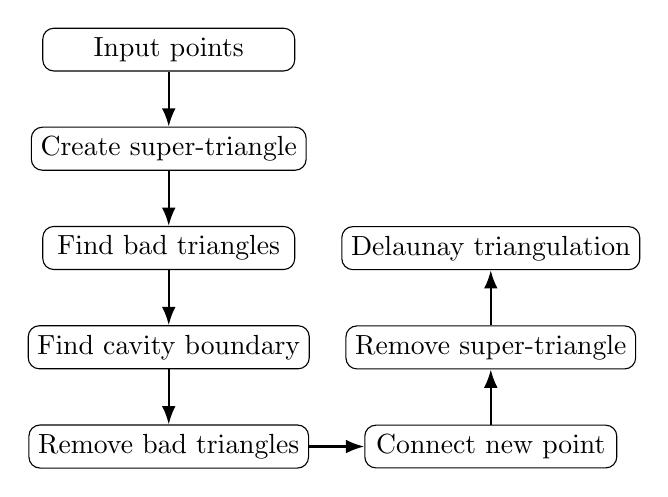
\begin{tikzpicture}[
    node distance=0.7cm,
    box/.style={
        rectangle,
        draw,
        rounded corners,
        minimum width=3.2cm,
        minimum height=0.5cm,
        align=center
    },
    arrow/.style={-{Latex}, thick}
]

\node[box] (input) {Input points};
\node[box, below=of input] (super) {Create super-triangle};
\node[box, below=of super] (bad) {Find bad triangles};
\node[box, below=of bad] (cavity) {Find cavity boundary};
\node[box, below=of cavity] (remove) {Remove bad triangles};
\node[box, right=of remove] (new) {Connect new point};
\node[box, above=of new] (clean) {Remove super-triangle};
\node[box, above=of clean] (output) {Delaunay triangulation};

\draw[arrow] (input)--(super);
\draw[arrow] (super)--(bad);
\draw[arrow] (bad)--(cavity);
\draw[arrow] (cavity)--(remove);
\draw[arrow] (remove)--(new);
\draw[arrow] (new)--(clean);
\draw[arrow] (clean)--(output);

\end{tikzpicture}
\end{center}

\end{frame}

%------------------------------------------------
\begin{frame}{Geometric Predicate: Orientation}

The orientation of three points is:

\[
\operatorname{orient}(a,b,c)
=
(b_x-a_x)(c_y-a_y)
-
(b_y-a_y)(c_x-a_x).
\]

\begin{itemize}
    \item $\operatorname{orient}>0$: counter-clockwise
    \item $\operatorname{orient}<0$: clockwise
    \item $\operatorname{orient}=0$: collinear
\end{itemize}

\begin{center}
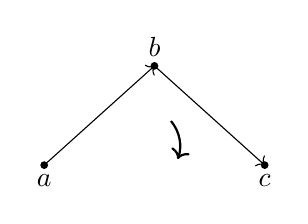
\begin{tikzpicture}[scale=0.7]

\coordinate (A) at (-2,0);
\coordinate (B) at (0,1.8);
\coordinate (C) at (2,0);

\draw[->] (A)--(B);
\draw[->] (B)--(C);

\fill (A) circle (2pt) node[below] {$a$};
\fill (B) circle (2pt) node[above] {$b$};
\fill (C) circle (2pt) node[below] {$c$};

\draw[->,thick] (0.3,0.8) arc (40:-20:0.7);

\end{tikzpicture}
\end{center}

Orientation is useful for robust geometric computations.

\end{frame}

%------------------------------------------------
\begin{frame}{Geometric Predicate: InCircle}

The second important predicate is:

\[
\operatorname{inCircle}(a,b,c,p).
\]

It determines whether $p$ lies inside the circumcircle of
triangle $(a,b,c)$.

For a counter-clockwise triangle:

\[
\det
\begin{pmatrix}
a_x & a_y & a_x^2+a_y^2 & 1\\
b_x & b_y & b_x^2+b_y^2 & 1\\
c_x & c_y & c_x^2+c_y^2 & 1\\
p_x & p_y & p_x^2+p_y^2 & 1
\end{pmatrix}
>0
\]

indicates that $p$ is inside the circumcircle.

\vspace{0.2cm}

\begin{block}{Implementation note}
Robust Delaunay implementations often use exact or adaptive-precision
geometric predicates rather than simple floating-point calculations.
\end{block}

\end{frame}

%------------------------------------------------
\begin{frame}[fragile]{Data Structures}

A simple implementation can represent points, edges, and triangles as:

\begin{lstlisting}[language=C++,basicstyle=\ttfamily\small]
struct Point {
    double x, y;
};

struct Edge {
    Point *a;
    Point *b;
};

struct Triangle {
    Point *a;
    Point *b;
    Point *c;
};
\end{lstlisting}

Important operations include:

\begin{itemize}
    \item \texttt{inCircle()}
    \item \texttt{orientation()}
    \item Finding cavity boundary edges
    \item Inserting new triangles
    \item Removing triangles
\end{itemize}

\end{frame}

%------------------------------------------------
\begin{frame}[fragile]{Core Implementation Logic}

\begin{lstlisting}[language=C++,basicstyle=\ttfamily\scriptsize]
for (Point *p : points) {

    vector<Triangle*> bad;

    // Find triangles whose circumcircle contains p
    for (Triangle *t : triangles) {
        if (inCircle(*p, *t))
            bad.push_back(t);
    }

    vector<Edge> boundary;

    // Find cavity boundary
    for (Triangle *t : bad) {
        for (Edge e : edges(t)) {

            if (countEdge(e, bad) == 1)
                boundary.push_back(e);
        }
    }

    // Remove bad triangles
    removeTriangles(bad);

    // Retriangulate cavity
    for (Edge e : boundary) {
        triangles.push_back(
            new Triangle{e.a, e.b, p}
        );
    }
}
\end{lstlisting}

\end{frame}

%------------------------------------------------
\begin{frame}{Complexity}

For a straightforward implementation:

\[
\boxed{O(n^2)}
\]

is a typical worst-case complexity.

Why?

\begin{itemize}
    \item There are $n$ point insertions.
    \item Each insertion may inspect many existing triangles.
    \item Finding the cavity can therefore take $O(n)$ work.
\end{itemize}

With appropriate spatial data structures and point-location methods,
the practical performance can be significantly improved.

\vspace{0.3cm}

\begin{block}{Key observation}
The triangulation is updated locally around the newly inserted point.
\end{block}

\end{frame}

%------------------------------------------------
\begin{frame}{Why Bowyer--Watson is Attractive}

\begin{columns}

\begin{column}{0.48\textwidth}

\textbf{Advantages}

\begin{itemize}
    \item Conceptually simple
    \item Incremental
    \item Local cavity updates
    \item Easy to implement
    \item Natural geometric interpretation
    \item Useful for mesh generation
\end{itemize}
\end{column}
\begin{column}{0.48\textwidth}

\textbf{Challenges}

\begin{itemize}
    \item Point insertion is sequential
    \item Robust predicates are important
    \item Naive implementation can be $O(n^2)$
    \item Cavity searches can be expensive
    \item Parallel insertion requires conflict handling
\end{itemize}
\end{column}
\end{columns}

\end{frame}

%------------------------------------------------
\begin{frame}{Parallelization Challenge}

The basic algorithm is inherently incremental:
\[
p_1
\rightarrow
p_2
\rightarrow
p_3
\rightarrow
\cdots
\rightarrow
p_n
\]

Each insertion modifies the triangulation.

\vspace{0.4cm}

However, multiple points may sometimes have \textbf{independent cavities}.

\begin{center}
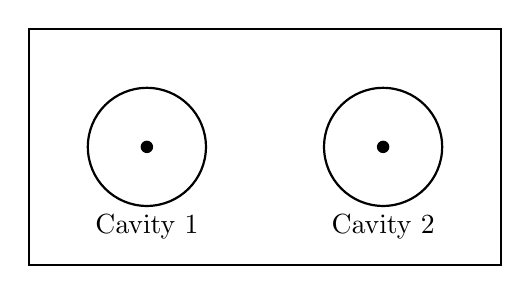
\begin{tikzpicture}[scale=0.75]

\draw[thick] (-4,-2) rectangle (4,2);

% Cavity 1
\draw[thick] (-2,0) circle (1);
\fill (-2,0) circle (3pt);
\node at (-2,-1.35) {Cavity 1};

% Cavity 2
\draw[thick] (2,0) circle (1);
\fill (2,0) circle (3pt);
\node at (2,-1.35) {Cavity 2};

\end{tikzpicture}
\end{center}

If the cavities do not overlap, their updates may be performed concurrently.

\end{frame}
%------------------------------------------------
\begin{frame}{Parallel Bowyer--Watson: Basic Idea}

A possible parallel approach is:

\begin{enumerate}
    \item Select a batch of points.
    \item Compute their cavities in parallel.
    \item Detect overlapping/conflicting cavities.
    \item Process independent cavities concurrently.
    \item Merge the resulting triangulations.
\end{enumerate}

\begin{center}
\[
\boxed{
\text{Points}
\rightarrow
\text{Parallel cavity detection}
\rightarrow
\text{Conflict detection}
\rightarrow
\text{Parallel updates}
}
\]
\end{center}
\vspace{0.4cm}

This is an important direction for GPU and multicore implementations.

\end{frame}
%------------------------------------------------
\begin{frame}{Applications}

Delaunay triangulation is used in:

\begin{itemize}
    \item Computational geometry
    \item Finite-element mesh generation
    \item Geographic information systems
    \item Terrain modeling
    \item Computer graphics
    \item Collision and proximity algorithms
    \item Voronoi diagram construction
    \item Scientific visualization
\end{itemize}

\vspace{0.3cm}

The Delaunay triangulation and Voronoi diagram are geometric duals.

\[
\boxed{
\text{Delaunay triangulation}
\quad\longleftrightarrow\quad
\text{Voronoi diagram}
}
\]

\end{frame}

%------------------------------------------------
\begin{frame}{Summary}

\begin{enumerate}
    \item Start with a large super-triangle.
    \item Insert points incrementally.
    \item Find triangles whose circumcircles contain the new point.
    \item Remove these bad triangles.
    \item Extract the boundary of the resulting cavity.
    \item Connect the new point to every boundary edge.
    \item Remove triangles connected to the super-triangle.
\end{enumerate}

\vspace{0.4cm}

\begin{block}{Central idea}
A new point invalidates a local set of triangles. Remove those
triangles and retriangulate the resulting cavity.
\end{block}

\[
\boxed{\text{Bowyer--Watson = Local cavity removal + retriangulation}}
\]

\end{frame}

%------------------------------------------------
\begin{frame}{Possible Next Step}

\begin{center}
\Large
\textbf{Parallel Delaunay Triangulation}
\end{center}

\vspace{0.5cm}

Interesting directions:

\begin{itemize}
    \item Multicore Bowyer--Watson
    \item GPU-based Delaunay triangulation
    \item CUDA cavity detection
    \item Parallel conflict detection
    \item Divide-and-conquer Delaunay triangulation
    \item Incremental Delaunay on GPU
    \item FPGA implementation
\end{itemize}

\end{frame}
\end{document}
